\chapter{SymPy}

\href{https://es.wikipedia.org/wiki/SymPy}{SymPy} es una biblioteca de
Python que permite realizar cálculos simbólicos. Nos ofrece las
capacidades de álgebra computacional, y se puede usar en línea a través
de \href{http://live.sympy.org/}{SymPy Live} o
\href{http://www.sympygamma.com/}{SymPy Gamma}, este último es similar a
\href{https://www.wolframalpha.com/}{Wolfram Alpha}.

Si usas Anaconda este paquete ya viene instalado por defecto pero si se
usa miniconda o pip debe instalarse.

\begin{listing}[H]
\begin{minted}[mathescape,
frame=lines,
framesep=2mm]{bash}
conda install sympy # Usando el gestor conda de
                    # Anaconda/Miniconda
pip install sympy # Usando el gestor pip (puede requerir
                  # instalar más paquetes)
\end{minted}
\end{listing}

Lo primero que debemos hacer, antes de usarlo, es importar el módulo,
como con cualquier otra biblioteca de Python.

Si deseamos usar SymPy de forma interactiva usamos

\begin{listing}[H]
\begin{minted}[mathescape,
frame=lines,
framesep=2mm]{python}
from sympy import *
init_printing()
\end{minted}
\end{listing}

Para scripting es mejor importar la biblioteca de la siguiente manera

\begin{listing}[H]
\begin{minted}[mathescape,
frame=lines,
framesep=2mm]{python}
import sympy as sym
\end{minted}
\end{listing}

Y llamar las funciones de la siguiente manera

\begin{listing}[H]
\begin{minted}[mathescape,
frame=lines,
framesep=2mm]{python}
x = sym.Symbols("x")
expr = sym.cos(x)**\DecValTok{2} + \DecValTok{3}*x
deriv = expr.diff(x)
\end{minted}
\end{listing}

en donde calculamos la derivada de \(\cos^2(x) + 3x\), que debe ser
\(-2\sin(x)\cos(x) + 3\).

\begin{listing}[H]
\begin{minted}[mathescape,
frame=lines,
framesep=2mm]{python}
%matplotlib notebook
import numpy as np
import matplotlib.pyplot as plt
from sympy import *
\end{minted}
\end{listing}

\begin{listing}[H]
\begin{minted}[mathescape,
frame=lines,
framesep=2mm]{python}
init_printing()
\end{minted}
\end{listing}

Definamos la variable \(x\) como un símbolo matemático. Esto nos permite
hacer uso de esta variable en SymPy.

\begin{listing}[H]
\begin{minted}[mathescape,
frame=lines,
framesep=2mm]{python}
x = symbols("x")
\end{minted}
\end{listing}

Empecemos con cálculos simples. Abajo, tenemos una \emph{celda de
código} con una suma. Ubica el cursor en ella y presiona SHIFT + ENTER
para evaluarla.

\begin{listing}[H]
\begin{minted}[mathescape,
frame=lines,
framesep=2mm]{python}
1 + 3
\end{minted}
\end{listing}

\[4\]

Realicemos algunos cálculos.

\begin{listing}[H]
\begin{minted}[mathescape,
frame=lines,
framesep=2mm]{python}
factorial(5)
\end{minted}
\end{listing}

\[120\]

\begin{listing}[H]
\begin{minted}[mathescape,
frame=lines,
framesep=2mm]{python}
1 // 3
\end{minted}
\end{listing}

\[0\]

\begin{listing}[H]
\begin{minted}[mathescape,
frame=lines,
framesep=2mm]{python}
1 / 3
\end{minted}
\end{listing}

\[0.3333333333333333\]

\begin{listing}[H]
\begin{minted}[mathescape,
frame=lines,
framesep=2mm]{python}
S(1) / 3
\end{minted}
\end{listing}

\[\frac{1}{3}\]

Podemos evaluar esta expresión a su versión en punto flotante

\begin{listing}[H]
\begin{minted}[mathescape,
frame=lines,
framesep=2mm]{python}
sqrt(2*pi)
\end{minted}
\end{listing}

\[\sqrt{2} \sqrt{\pi}\]

\begin{listing}[H]
\begin{minted}[mathescape,
frame=lines,
framesep=2mm]{python}
float(sqrt(2*pi))
\end{minted}
\end{listing}

\[2.5066282746310007\]

También podemos almacenar expresiones como variables, como cualquier
variable de Python.

\begin{listing}[H]
\begin{minted}[mathescape,
frame=lines,
framesep=2mm]{python}
radius = 10
height = 100
area = pi * radius**2
volume = area * height
\end{minted}
\end{listing}

\begin{listing}[H]
\begin{minted}[mathescape,
frame=lines,
framesep=2mm]{python}
volume
\end{minted}
\end{listing}

\[10000 \pi\]

\begin{listing}[H]
\begin{minted}[mathescape,
frame=lines,
framesep=2mm]{python}
float(volume)
\end{minted}
\end{listing}

\[31415.926535897932\]

Hasta ahora, hemos usado SymPy como una calculadora. Intentemos algunos
cálculos más avanzados. Por ejemplo, algunas integrales.

\begin{listing}[H]
\begin{minted}[mathescape,
frame=lines,
framesep=2mm]{python}
integrate(sin(x), x)
\end{minted}
\end{listing}

\[- \cos{\left (x \right )}\]

\begin{listing}[H]
\begin{minted}[mathescape,
frame=lines,
framesep=2mm]{python}
integrate(sin(x), (x, 0, pi))
\end{minted}
\end{listing}

\[2\]

Podemos definir una función, e integrarla

\begin{listing}[H]
\begin{minted}[mathescape,
frame=lines,
framesep=2mm]{python}
f = lambda x: x**2 + 5
\end{minted}
\end{listing}

\begin{listing}[H]
\begin{minted}[mathescape,
frame=lines,
framesep=2mm]{python}
f(5)
\end{minted}
\end{listing}

\[30\]

\begin{listing}[H]
\begin{minted}[mathescape,
frame=lines,
framesep=2mm]{python}
integrate(f(x), x)
\end{minted}
\end{listing}

\[\frac{x^{3}}{3} + 5 x\]

\begin{listing}[H]
\begin{minted}[mathescape,
frame=lines,
framesep=2mm]{python}
y = symbols("y")
integrate(1/(x**2 + y), x)
\end{minted}
\end{listing}

\[- \frac{\sqrt{- \frac{1}{y}}}{2} \log{\left (x - y \sqrt{- \frac{1}{y}} \right )} + \frac{\sqrt{- \frac{1}{y}}}{2} \log{\left (x + y \sqrt{- \frac{1}{y}} \right )}\]

Si asumimos que el denominador es positivo, esta expresión se puede
simplificar aún más

\begin{listing}[H]
\begin{minted}[mathescape,
frame=lines,
framesep=2mm]{python}
a = symbols("a", positive=True)
integrate(1/(x**2 + a), x)
\end{minted}
\end{listing}

\[\frac{1}{\sqrt{a}} \operatorname{atan}{\left (\frac{x}{\sqrt{a}} \right )}\]

Hasta ahora, aprendimos lo más básico. Intentemos algunos ejemplos más
complicados ahora.

\textbf{Nota:} Si quieres saber más sobre una función específica se
puede usar la función \texttt{help()} o el comándo \emph{mágico} de
IPython \texttt{??}

\begin{listing}[H]
\begin{minted}[mathescape,
frame=lines,
framesep=2mm]{python}
help(integrate)
\end{minted}
\end{listing}

\begin{verbatim}
  Help on function integrate in module sympy.integrals.integrals:

integrate(*args, **kwargs)
    integrate(f, var, ...)
    
    .
    .
    .
    
    >>> integrate(x**a*exp(-x), (x, 0, oo), conds='separate')
    (gamma(a + 1), -re(a) < 1)
    
    See Also
    ========
    
    Integral, Integral.doit
\end{verbatim}

El bloque de salida anterior fue resumido (indicación de los puntos verticales).

\begin{listing}[H]
\begin{minted}[mathescape,
frame=lines,
framesep=2mm]{python}
integrate??
\end{minted}
\end{listing}

\section{Ejemplos}

\hypertarget{soluciuxf3n-de-ecuaciones-algebraicas}{%
\subsection{Solución de ecuaciones
algebraicas}\label{soluciuxf3n-de-ecuaciones-algebraicas}}

Para resolver sistemas de ecuaciones algebraicos podemos usar:
\texttt{solveset} and \texttt{solve}
\textless{}\url{http://docs.sympy.org/latest/tutorial/solvers.html}\textgreater{}\_\_. El
método preferido es solveset, sin embargo, hay sistemas que se
pueden resolver usando solve` y no \texttt{solveset}.

Para resolver sistemas usando \texttt{solveset}:

\begin{listing}[H]
\begin{minted}[mathescape,
frame=lines,
framesep=2mm]{python}
a, b, c = symbols("a b c")
solveset(a*x**2 + b*x + c, x)
\end{minted}
\end{listing}

\[\left\{- \frac{b}{2 a} - \frac{1}{2 a} \sqrt{- 4 a c + b^{2}}, - \frac{b}{2 a} + \frac{1}{2 a} \sqrt{- 4 a c + b^{2}}\right\}\]

Debemos ingresar la expresión igualada a 0, o como una ecuación

\begin{listing}[H]
\begin{minted}[mathescape,
frame=lines,
framesep=2mm]{python}
solveset(Eq(a*x**2 + b*x, -c), x)
\end{minted}
\end{listing}

\[\left\{- \frac{b}{2 a} - \frac{1}{2 a} \sqrt{- 4 a c + b^{2}}, - \frac{b}{2 a} + \frac{1}{2 a} \sqrt{- 4 a c + b^{2}}\right\}\]

\texttt{solveset} no permite resolver sistemas de ecuaciones no
lineales, por ejemplo

\begin{listing}[H]
\begin{minted}[mathescape,
frame=lines,
framesep=2mm]{python}
solve([x*y - 1, x - 2], x, y)
\end{minted}
\end{listing}

\[\left [ \left ( 2, \quad \frac{1}{2}\right )\right ]\]

\subsection{Álgebra lineal}

Usamos \texttt{Matrix} para crear matrices. Las matrices pueden contener
variables y expresiones matemáticas.

Usamos el método \texttt{.inv()} para calcular la inversa, y \texttt{*}
para multiplicar matrices.

\begin{listing}[H]
\begin{minted}[mathescape,
frame=lines,
framesep=2mm]{python}
A = Matrix([
        [1, -1],
        [1, sin(c)]
    ])
display(A)
\end{minted}
\end{listing}

\[\begin{aligned}
\left[\begin{matrix}1 & -1\\1 & \sin{\left (c \right )}\end{matrix}\right]
\end{aligned}\]

\begin{listing}[H]
\begin{minted}[mathescape,
frame=lines,
framesep=2mm]{python}
B = A.inv()
display(B)
\end{minted}
\end{listing}

\[\begin{aligned}
\left[\begin{matrix}\frac{\sin{\left (c \right )}}{\sin{\left (c \right )} + 1} & \frac{1}{\sin{\left (c \right )} + 1}\\- \frac{1}{\sin{\left (c \right )} + 1} & \frac{1}{\sin{\left (c \right )} + 1}\end{matrix}\right]
\end{aligned}\]

\begin{listing}[H]
\begin{minted}[mathescape,
frame=lines,
framesep=2mm]{python}
A * B
\end{minted}
\end{listing}

\[\begin{aligned}
\left[\begin{matrix}\frac{\sin{\left (c \right )}}{\sin{\left (c \right )} + 1} + \frac{1}{\sin{\left (c \right )} + 1} & 0\\0 & \frac{\sin{\left (c \right )}}{\sin{\left (c \right )} + 1} + \frac{1}{\sin{\left (c \right )} + 1}\end{matrix}\right]
\end{aligned}\]

Esta expresión debería ser la matriz identidad, simplifiquemos la
expresión. Existen varias formas de simplificar expresiones, y
\texttt{simplify} es la más general.

\begin{listing}[H]
\begin{minted}[mathescape,
frame=lines,
framesep=2mm]{python}
simplify(A * B)
\end{minted}
\end{listing}

\[\begin{aligned}
\left[\begin{matrix}1 & 0\\0 & 1\end{matrix}\right]
\end{aligned}\]

\subsection{Graficación}

SymPy permite realizar gráficos 2D y 3D

\begin{listing}[H]
\begin{minted}[mathescape,
frame=lines,
framesep=2mm]{python}
from sympy.plotting import plot3d
\end{minted}
\end{listing}

\begin{listing}[H]
\begin{minted}[mathescape,
frame=lines,
framesep=2mm]{python}
plot(sin(x), (x, -pi, pi));
\end{minted}
\end{listing}

\begin{figure}[H]
	\centering
	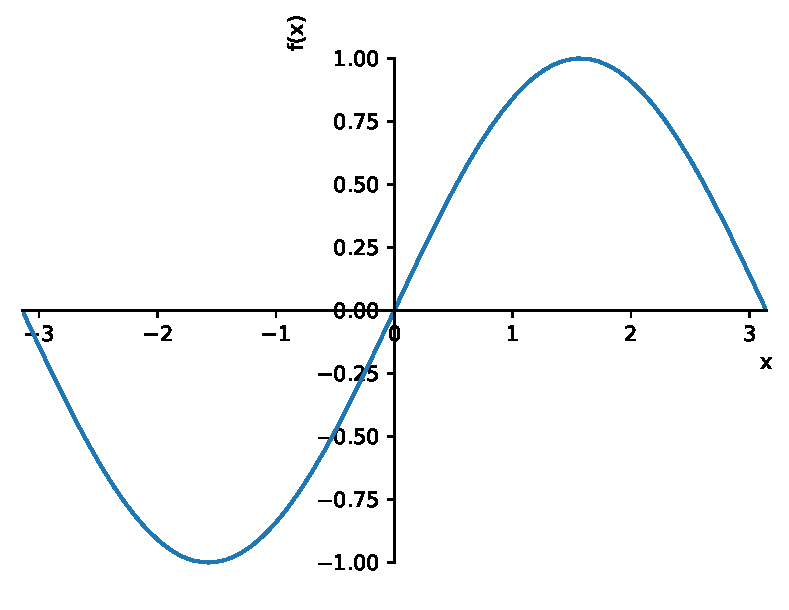
\includegraphics[width=10cm]{img/sympy/sympy_grafico}
	\caption{Ejemplo de gráfico con SymPy.}
	\label{fig:grafico_sympy}
\end{figure}

\begin{listing}[H]
\begin{minted}[mathescape,
frame=lines,
framesep=2mm]{python}
monkey_saddle = x**3 - 3*x*y**2
p = plot3d(monkey_saddle, (x, -2, 2), (y, -2, 2))
\end{minted}
\end{listing}

\begin{figure}[H]
	\centering
	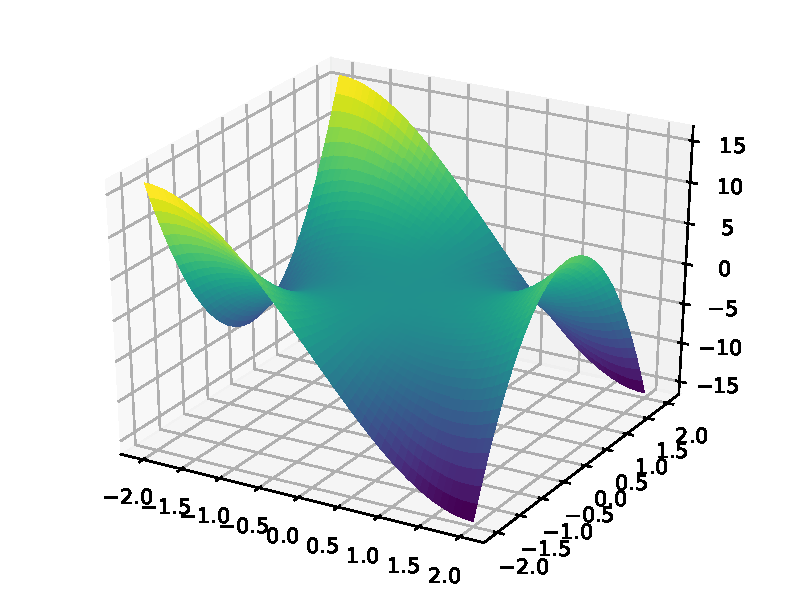
\includegraphics[width=10cm]{img/sympy/sympy_grafico_3D}
	\caption{Ejemplo de gráfico 3D con sympy.}
	\label{fig:grafico_sympy_3D}
\end{figure}

\hypertarget{derivadas-y-ecuaciones-diferenciales}{%
\subsection{Derivadas y ecuaciones
diferenciales}\label{derivadas-y-ecuaciones-diferenciales}}

Podemos usar la función \texttt{diff} o el método \texttt{.diff()} para
calcular derivadas.

\begin{listing}[H]
\begin{minted}[mathescape,
frame=lines,
framesep=2mm]{python}
f = lambda x: x**2
\end{minted}
\end{listing}

\begin{listing}[H]
\begin{minted}[mathescape,
frame=lines,
framesep=2mm]{python}
diff(f(x), x)
\end{minted}
\end{listing}

\[2 x\]

\begin{listing}[H]
\begin{minted}[mathescape,
frame=lines,
framesep=2mm]{python}
f(x).diff(x)
\end{minted}
\end{listing}

\[2 x\]

\begin{listing}[H]
\begin{minted}[mathescape,
frame=lines,
framesep=2mm]{python}
g = lambda x: sin(x)
\end{minted}
\end{listing}

\begin{listing}[H]
\begin{minted}[mathescape,
frame=lines,
framesep=2mm]{python}
diff(g(f(x)), x)
\end{minted}
\end{listing}

\[2 x \cos{\left (x^{2} \right )}\]

Y sí, ¡SymPy sabe sobre la regla de la cadena!

Para terminar, resolvamos una ecuación diferencial de segundo orden

\[u''(t) + \omega^2 u(t) = 0\]

\begin{listing}[H]
\begin{minted}[mathescape,
frame=lines,
framesep=2mm]{python}
t = symbols("t")
u = symbols("u", cls=Function)
omega = symbols("omega", positive=True)
\end{minted}
\end{listing}

\begin{listing}[H]
\begin{minted}[mathescape,
frame=lines,
framesep=2mm]{python}
ode = u(t).diff(t, 2) + omega**2 * u(t)
dsolve(ode, u(t))
\end{minted}
\end{listing}

\[u{\left (t \right )} = C_{1} \sin{\left (\omega t \right )} + C_{2} \cos{\left (\omega t \right )}\]

\hypertarget{convertir-expresiones-de-sympy-en-funciones-de-numpy}{%
\section{Convertir expresiones de SymPy en funciones de
NumPy}\label{convertir-expresiones-de-sympy-en-funciones-de-numpy}}

\texttt{lambdify} permite convertir expresiones de sympy en funciones
para hacer cálculos usando NumPy.

Veamos cómo.

\begin{listing}[H]
\begin{minted}[mathescape,
frame=lines,
framesep=2mm]{python}
f = lambdify(x, x**2, "numpy")
f(3)
\end{minted}
\end{listing}

9

\begin{listing}[H]
\begin{minted}[mathescape,
frame=lines,
framesep=2mm]{python}
f(np.array([1, 2, 3]))
\end{minted}
\end{listing}

array({[}1, 4, 9{]})

Intentemos un ejemplo más complejo

\begin{listing}[H]
\begin{minted}[mathescape,
frame=lines,
framesep=2mm]{python}
fun = diff(sin(x)*cos(x**3) - sin(x)/x, x)
fun
\end{minted}
\end{listing}

\[- 3 x^{2} \sin{\left (x \right )} \sin{\left (x^{3} \right )} + \cos{\left (x \right )} \cos{\left (x^{3} \right )} - \frac{1}{x} \cos{\left (x \right )} + \frac{1}{x^{2}} \sin{\left (x \right )}\]

\begin{listing}[H]
\begin{minted}[mathescape,
frame=lines,
framesep=2mm]{python}
fun_numpy = lambdify(x, fun, "numpy")
\end{minted}
\end{listing}

y evalúemoslo en algún intervalo, por ejemplo, \([0, 5]\).

\begin{listing}[H]
\begin{minted}[mathescape,
frame=lines,
framesep=2mm]{python}
pts = np.linspace(0, 5, 1000)
fun_pts = fun_numpy(pts + 1e-6) # Para evitar división por 0
\end{minted}
\end{listing}

\begin{listing}[H]
\begin{minted}[mathescape,
frame=lines,
framesep=2mm]{python}
plt.figure()
plt.plot(pts, fun_pts)
\end{minted}
\end{listing}

\begin{figure}[H]
	\centering
	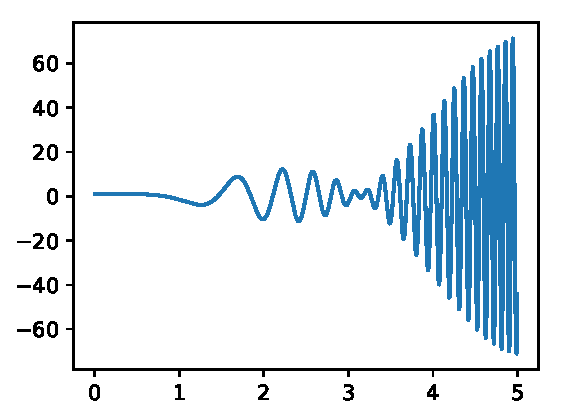
\includegraphics[width=10cm]{img/sympy/sympy_lambdify}
	\caption{Gráfico de la función evaluada luego de usar lambdify.}
	\label{fig:grafico_lambdify}
\end{figure}

\section{Ejercicios}

\begin{enumerate}
\def\labelenumi{\arabic{enumi}.}
\item
  Calcule el límite
\end{enumerate}

\[\lim_{x \rightarrow 0} \frac{\sin(x)}{x}\, .\]

\begin{enumerate}
\def\labelenumi{\arabic{enumi}.}
\setcounter{enumi}{1}
\item
  Resuelva la ecuación diferencial de Bernoulli
\end{enumerate}

\[x \frac{\mathrm{d} u(x)}{\mathrm{d}x}  + u(x) - u(x)^2 = 0\, .\]

\section{Recursos adicionales}

\begin{itemize}
\item Equipo de desarrollo de SymPy. \href{http://docs.sympy.org/latest/tutorial/index.html}{SymPy Tutorial}, (2018). Consultado: Julio 23, 2018

\item Ivan Savov. \href{https://minireference.com/static/tutorials/sympy_tutorial.pdf}{Taming math and physics using SymPy}, (2017). Consultado: Julio 23, 2018



\end{itemize}
